\section{Security Protocols} % Message deduction?
Security protocols is an abstract or concrete protocol, that characterise the security related functions and applies cryptographic methods. It describes how the algorithm should be used to ensure the security and integrity of data transmitted. The security protocol is a protocol that runs in an untrusted environment, where it usually assumes channels are untrusted and participants are dishonest. In academic examples, they are often described with the Alice and Bob notation, which will also be used in the following examples. (The Dolev-Yao model) 

%A way of reason about wether a message is deductible by an adversary is through inference rules. Inference rules offers a formal analysis for proving security properties of protocols. \\ \\
%TODO: discuss how Inference rules and derivation sequences can be used 

\subsection{Needham-Schroeder Protocol}
The Needham-Schroeder Public Key Protocol, was first proposed by Roger Needham and Michael Schroeder in 1978 (ref?), and will be used as a running example in this and the following two sections. %and is one of the two key transport protocols intended for an insecure network. 

The Needham-Schroeder Public Key Protocol can be illustrated by the before mentioned Alice and Bob notation in the following way, as done by \citeauthor{DBLP:journals/ftpl/CortierK14}

\begin{center}
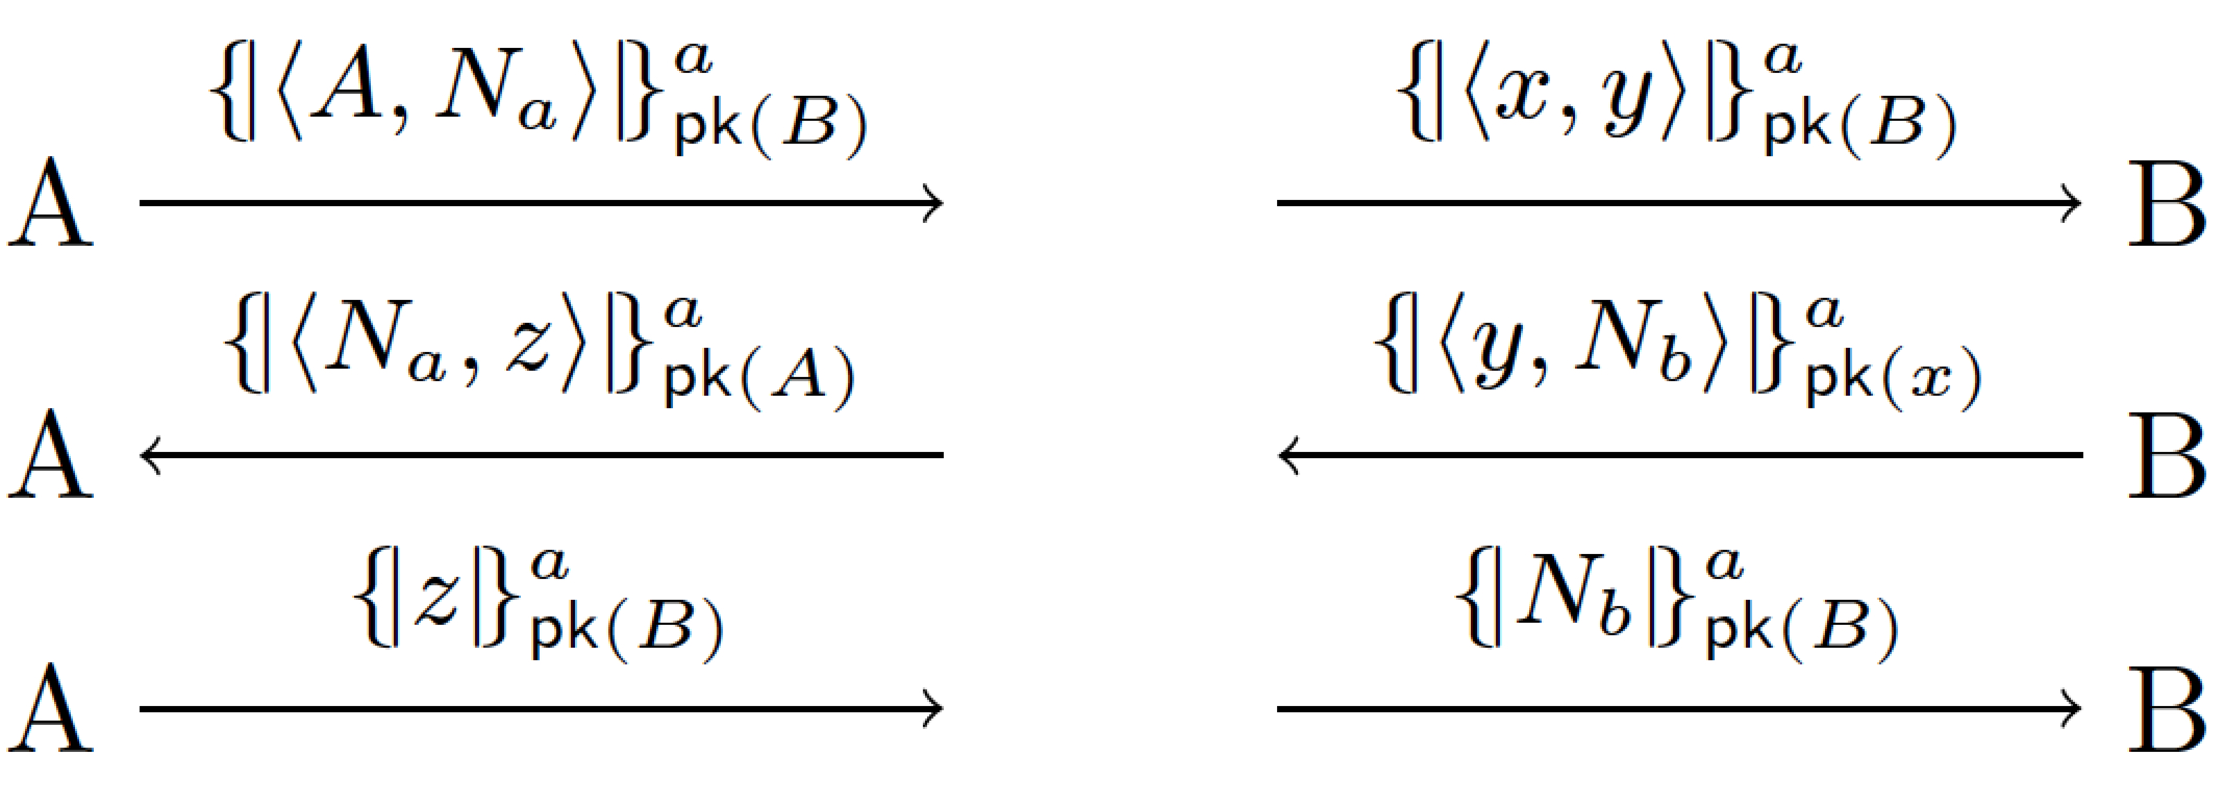
\includegraphics[width=0.7\textwidth, angle=0]{Graphics/NS_Protocol.pdf}
\end{center}

The A and B each represent Alice and Bob, while the arrows indicates the direction of the sent and received messages, by which are illustrated above each line. The notation $\{| m |\}^a_{pk(B)}$ denotes that the message \textit{m} is created with an asymmetric encryption of Bob's public key, while the $\langle m_1, m_2 \rangle$ illustrates a pairing, so a concatenation of the two messages. 
\\ \\The cap left between the two participants, is to illustrate the challenge of this protocol, and will be addressed later in the report. 

\iffalse
A -> B : m  			= Alice sends Bob a message
Notation {|m|}^a_pk(B) 	= asymmetric encryption of m with Bob's public key. 
<m1, m2>				= pairing, i.e. concatenation of the two messages
A, B					= Their identities
N_a					= nonce (number used once - fresh random generated each session)
First 					= Alice sends her identity and nonce, encrypted with Bob's public key

Bob then decrypts and check that it is well-formed.
This mechanism of sending someone an encrypted nonce and waiting for the recipient to send back this nonce is often called a challenge-response mechanism.
Alice then decrypts Bob's message, and verifies that it contains har previous N_a - proves that Bob received first message

The aim of the protocol is to guarantee mutual 'authentication' - ensures they have been communicating with the right person
Moreover, the protocol should guarantee 'confidentiality' of the nonces Na and Nb.
 - Honest execution (man in the middle attack)
\fi

\subsection{Message deduction}
TODO: Deduction rules \\
TODO: Derivation sequence

%\subsection{Examples}
%TODO: show examples of a man in the middle attack on the NS and DH protocols: \\ \\
%- Needham-Schroeder Public key protocol (now modified according to Lowe's man in the middle attack): 


